\section{Profiling}
\label{sec:profiling}
The space and timing complexity of any application is measured by the profiling. In this assignment, MCProf profiling tool is being used for profiling of the  \emph{Canny Edge Detection} application. MCProf is a runtime Memory and Communication profiler which generates detailed application profile in terms of memory access patterns and data-communication at function and loop-level granularity. Profiling of this application was performed for the given set of sample pictures and the results showed us that the \emph{gaussian-smooth} function consumes almost 80\% of the processing time for each input picture. Moreover, most of the memory accesses are also done by this function. Therefore, this function has become the center of our attention and was subject to acceleration. The profiling result with the \emph{tiger.pgm} as an input image is shown in figure~\ref{fig:prof}. Note that the input image has very little impact on the results' deviations.



\textit{The profiling results of the rest of the pictures are attached in the appendix}


\begin{figure}
\centering
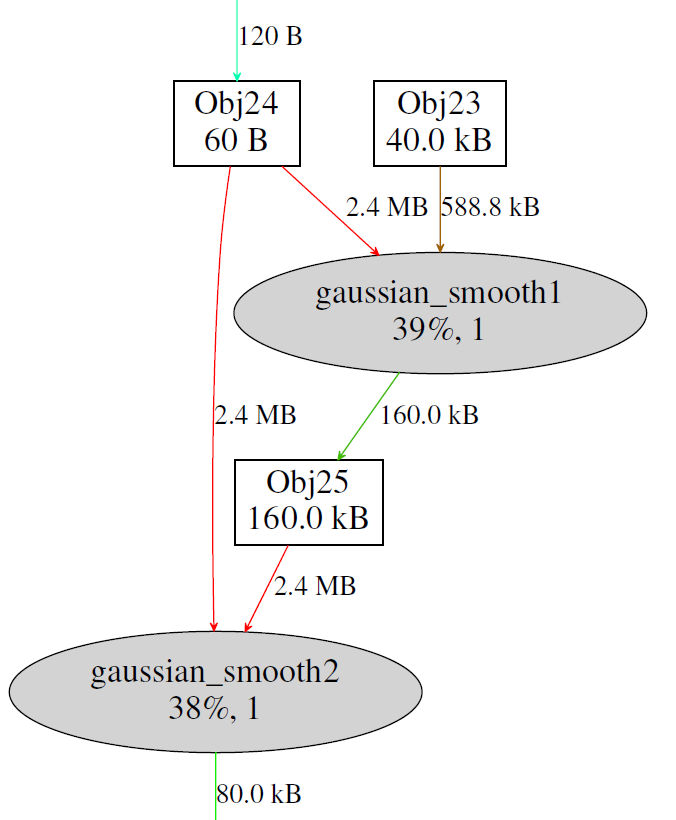
\includegraphics[width=0.4\textwidth]{tiger_profile}
\caption{Application profiling for \textit{tiger.png}. \textit{Some output omitted for brevity}}
\label{fig:prof}
\end{figure}